\section{实验评估}
\label{sec:experiments_lifelong}

本节中，我们将在一组终身 \gls{rl} 任务中测试 POLIS 与不同基线方法的性能。
第一组实验将考虑无延迟的非平稳环境，以评估算法面对动态变化的能力。
然后，第二组实验将考虑在先前任务中添加延迟，以评估 POLIS 对延迟的鲁棒性。
在本节中，我们将对我们关注的终身 \gls{rl} 中 \glspl{mdp} 的特定情况做一个假设。
该假设是智能体无法通过其动作影响状态的一部分，且只有这部分状态可以是非平稳的。
例如，这在金融数学中是简化分析的常见假设。
通常假设仅交易小规模投资头寸不会影响市场动态。
这大大简化了实验设置，并允许更清晰地评估我们的算法面对可观测非平稳性的能力。
该假设正式表述如下。
\begin{ass}
    \label{ass:factorable_state}
转移模型 $\markovchaintransition= (\markovchaintransition_t)_{t \in \naturalnumbers}$ 分解如下，对于任意 $x = (x^c,x^u) \in \statespace$，$a \in \actionspace$，和 $t \in \naturalnumbers$：
\begin{equation}
    \markovchaintransition_t(x'\vert x,a) = \markovchaintransition^c({x'}^c\vert x^c,x^u,a) \markovchaintransition_t^u({x'}^u\vert x^u) .
\end{equation}
\end{ass}

除该假设外，在下面考虑的任务中，$\markovchaintransition^c$ 是确定性的。
这使得我们可以通过使用新策略采样状态的可控部分来获得 $\alpha$ 步后视期望回报的值，同时状态的非平稳部分 $x^u$ 保持不变。
因此，我们可以获得 $\alpha$ 步后视期望回报梯度的精确值，而不需要重要性采样。

接下来，我们在 \Cref{subsec:setting_exp_lifelong} 中描述实验设置，然后在 \Cref{subsec:results_lifelong} 中提供结果。


\subsection{设置}
\label{subsec:setting_exp_lifelong}


\subsubsection{任务}
首先，我们描述终身学习的一般背景。
与环境的终身交互时间表可以分为两个阶段。
在第一个阶段，我们称为 \emph{行为阶段}，行为超策略从环境中采样数据。
这是收集足够数据以计算替代目标中使用的第一个 {$\alpha$ 步后视期望回报}所必需的。
然后，在第二个阶段，智能体从行为超策略停止的位置继续与环境交互。然而，它现在可以定期重新训练其超策略。
在实践中，我们在所有测试环境中每 50 步重新训练一次。
每次进行 100 步梯度更新。
我们将此阶段称为 \emph{目标阶段}。
对于所有任务，我们设置 $\gamma=\omega=1$。

\noindent\textbf{无延迟 EUR-USD 交易.}\indent 第一个任务类似于 \Cref{subsubsec:tasks_imitation} 中的交易任务。
它也考虑在外汇市场上交易 EUR-USD（\texteuro/\$）货币对，但这次是基于日数据。
智能体可以选择 $[-1,1]$ 中的连续动作；$1$ 和 $-1$ 对应以最大订单规模 10 万美元买入或卖出，而动作 $0$ 对应保持空仓。
在 \Cref{ass:factorable_state} 下，我们假设最大订单规模相对于可用市场流动性很小，因此对市场动态没有影响。
智能体观测到的状态由其当前投资组合（$x_{t}^{c}$）组成，即其先前动作的价值和当前货币汇率（$x_{t}^{u}$）。
我们将历史数据分为三个数据集：2009-2012、2013-2016 和 2017-2020；每个时期有略多于 $1000$ 个数据点。
各时期的历史利率见 \Cref{subsubsec:datasets_lifelong}。
奖励定义为 $r_{t}=a_t(x_{t+1}^{u}-x_{t}^{u})-f\lvert a_t - x_{t}^{c}\rvert$，其中 $f$ 是费用，相当于投资规模的 $1\mathrm{e}{-3}\;\%$。
我们设置 $\alpha$ 为 500，同时考虑 500 步的目标阶段。
需要注意的是，由于终身学习框架中训练和测试之间没有明确区分，选择超参数（指 POLIS 参数，而非超策略）可能很复杂。
通过在目标阶段评估性能来选择最佳超参数是危险的，因为如果目标阶段被延长，显然会过拟合并泛化不良。
为了研究这个问题，我们对此任务比较两种超参数选择方案。
对于第一种方案，我们在 2009-2012 数据集的目标阶段选择超参数，并在其他两个数据集上评估。
在第二种方案中，我们在最后两个数据集的目标阶段同时选择超参数和评估。

\noindent\textbf{无延迟 Vasicek 交易.}\indent 由于 EUR-USD 货币对是一种高度复杂的资产，我们考虑交易一种具有更平滑非平稳性的合成利率，以为智能体提供更好的信噪比。
我们保留整体交易框架，仅修改汇率 $(x_{t}^{c})_{t\ge0}$，将历史 EUR-USD 利率替换为 Vasicek 过程。
框架的其他部分保持不变。
所考虑的 Vasicek 过程为 $x_{t+1}^{c} = 0.9 x_{t}^{c} + u_t$，其中 $u_t\sim\mathcal{N}(0,1)$。

\noindent\textbf{无延迟水坝.}\indent 第三个任务考虑水资源管理问题，其中水坝用于控制湖泊水位。
湖泊从某些入流（如雨水）获得水，而水坝控制其出流。
目标是利用出水满足一定需求（如城镇供水），即使在干旱时期也是如此。
这涉及在预期降雨时储水，同时避免洪水。
我们使用来自 \cite{castelletti2010tree, pmlr-v80-tirinzoni18a} 的环境模型。
考虑三种不同的随机年入流量\footnote{其均值在 \Cref{subsubsec:datasets_lifelong} 中给出}。
智能体对它们没有影响，满足 \Cref{ass:factorable_state}。
作为状态，智能体观测当前日期的湖泊水位。
对 \cite{castelletti2010tree, pmlr-v80-tirinzoni18a} 原始设定的唯一修改是智能体不观测年份中的日期，以确保非平稳性。
否则，智能体可以学习将年份中的日期映射到其期望入流，这将使问题回到平稳设定。
动作空间是连续的。
我们考虑洪水水位 $F=300$ 和每日需水量 $D=10$。
对于某个湖泊水位 $x$ 和某个选择的出流（或动作）$a$，未满足需求的惩罚为 $c_D = (\max(a-D,0))^2$，洪水的额外惩罚为 $c_F = (\max(x-F,0))^2$。
总成本根据入流情况通过加权这两种成本来组合这些惩罚，详见 \Cref{subsubsec:datasets_lifelong}。
为了更好地理解过程动态，我们将 $\alpha$ 设置为 1000，以便估计器使用足够多的过去数据。
我们将目标阶段的长度设置为 500 步。
关于超参数，在该环境中结果对超参数选择似乎不太敏感，因此我们仅基于第一个入流情况选择超参数。
% AS we will see in the results, it may be necessary to change the frequency of retraining to have longer periods without updates in order to amplify the necessity to adapt to non-stationary.

\noindent\textbf{延迟 Vasicek 交易.}\indent 该任务与之前的 Vasicek 交易任务相同，但增加了延迟。
我们考虑 $\delay$ 在 $[\![1,10]\!]$ 范围内的延迟，以研究延迟增加对回报的影响。
如本章所述，在此智能体是无记忆的。
看到历史汇率 $x_{t-\delay}$ 及其在时间 $t-\delay$ 的投资组合后，智能体选择一笔交易，该交易将以汇率 $x_t$ 执行，并考虑其在时间 $t$ 的当前投资组合。
因此，POLIS 学习的策略必须跟踪其投资组合以及过程的非平稳性，以选择其下一笔交易。

\noindent\textbf{延迟水坝.}\indent 在该环境中，我们考虑上述水资源管理任务。
与延迟 Vasicek 交易一样，我们测试 POLIS 在递增延迟下的表现，以评估其在该环境中的鲁棒性。

\subsubsection{基线方法}
第一个明显的基线是平稳策略。
它可以视为 POLIS 的特例，其中超策略随时间恒定 $\nu_{\boldsymbol\rho}(\cdot\vert t)=\nu_{\boldsymbol\rho}(\cdot)$。
为了突出 POLIS 方法的效果，我们考虑这样一个平稳超策略 $\nu_{\boldsymbol\rho}$，其结构和优化与 POLIS 完全相同，只是去除了方差惩罚和对时间的依赖。
但需要注意的是，尽管在重新训练步骤之间是平稳的，但平稳策略的参数也每 50 步重新训练一次，与 POLIS 和其他基线方法相同。
在此基线之上，我们还考虑了文献中的几种方法，包括 Pro-OLS 和 Pro-WLS~\cite{chandak2020optimizing}；+、LPG-FTW~\cite{mendez2020lifelong} 和 ONPG（\cite{chandak2020optimizing} 在其实验中提到的作为 \cite{al-shedivat2018continuous} 思想复制的基线方法）。


\subsubsection{POLIS 的设置}
在本小节中，我们更精确地描述 POLIS 内部使用的策略和超策略。
我们的超策略由两个模块组成。
第一个模块是 \cite{vaswani2017attention} 中引入的 \emph{位置编码}（见 \Cref{subsubsec:transformer}）。
在这里使用它有两个原因。首先，其输出维度是一个超参数，因此可用于控制下一模块的输入维度。
其次，虽然时间索引可以无限增长，但位置编码的输出是有界的。
这在将该值馈入 \glsfirst{nn} 时尤其有用。
第二个模块 \emph{时间卷积}~\cite{oord2016wavenet} 用于随时间扫描其输入。
卷积的一个主要优点是它们通常擅长在序列中发现模式 \cite{liotet2020deep}。
另一个优点是它们的通用性，它们接受不同长度的输入，并且可以有效并行化。
由于它们的 \emph{感受野}（即卷积支撑集的大小），位置编码层应提供比最后一个时间 $t$ 更多的输入。
这可以通过将较旧的时间步与 $t$ 一起作为输入序列来实现。
这一修改并不否定超策略仅依赖当前时间 $t$ 的观点。
感受野的长度为 $b=2^{l-1}(k-1)$，其中 $l$ 和 $k$ 分别是时间卷积的层数和卷积核大小。
作为时间 $t$ 的输出，时间卷积返回正态分布的均值 $\boldsymbol{\mu}_t$，策略参数 $\boldsymbol\theta_t$ 从中采样。
我们选择将这些正态分布的标准差限制为不依赖于时间，但可以在终身交互过程中每 50 步重新训练或固定不变。
超策略的图形表示见 \Cref{fig:hyper_policy_polis}。
如上所述，时间卷积的一个巨大优势是可以并行采样未来 $N$ 个策略参数 $(\boldsymbol\theta_i)_{i\in[\![t,t+N]\!]}$，对于任意 $N>0$。
只需将时间 $[\![t-b,t+N]\!]$ 馈入超策略即可获得这些参数。

最后，在策略层面，我们考虑一个具有有界输出的简单仿射策略。
平稳基线方法也是如此。

\begin{figure}[t]
    \centering
    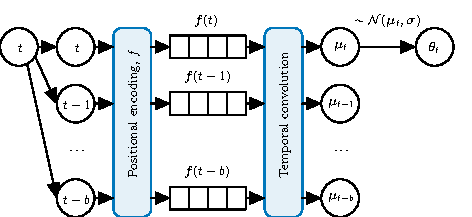
\includegraphics[labellifelongtrading=hyperpolicypolis]{img/thesis_plots_chapter_lifelong_trading.pdf}
    \caption{超策略在时间 $t$ 被查询时的图形表示。
    首先，由于时间卷积具有长度为 $b$ 的感受野，我们将最后 $b$ 个时间追加到 $t$，作为馈入位置编码的输入。
    后者为每个时间输出一个向量 $\boldsymbol{f}(t)$。
    这些向量随后被馈入时间卷积，该卷积返回每个策略参数 $\boldsymbol\theta_k$ 在时间 $k$ 的均值 $\boldsymbol{\mu}_k$。
    其中最后一个就是当前策略参数 $\boldsymbol\theta_t$。}
    \label{fig:hyper_policy_polis}
\end{figure}


\subsection{结果}
\label{subsec:results_lifelong}

\noindent\textbf{无延迟 EUR-USD 交易.}\indent 我们在 \Cref{fig:trading_eurusd} 中报告了随时间累积回报的结果。
在上图中，超参数在训练集（2009-2012）上选择。
有趣的是，对于 2013-2016 时期，平稳策略取得了最佳性能，而 POLIS 具有非常相似的性能。
然而，回顾一下，平稳策略仅是在重新训练步骤之间是平稳的。
2017-2020 时期似乎更为复杂，因为没有方法获得正回报。
POLIS 的表现低于大多数基线方法，但优于平稳策略。
在下图中，超参数在测试集（2013-2016 和 2017-2020 合并）上选择。
在这些测试中，POLIS 的性能与其他基线方法更为相似，没有方法明显优于其他方法。

\begin{figure}[t]
    \centering
    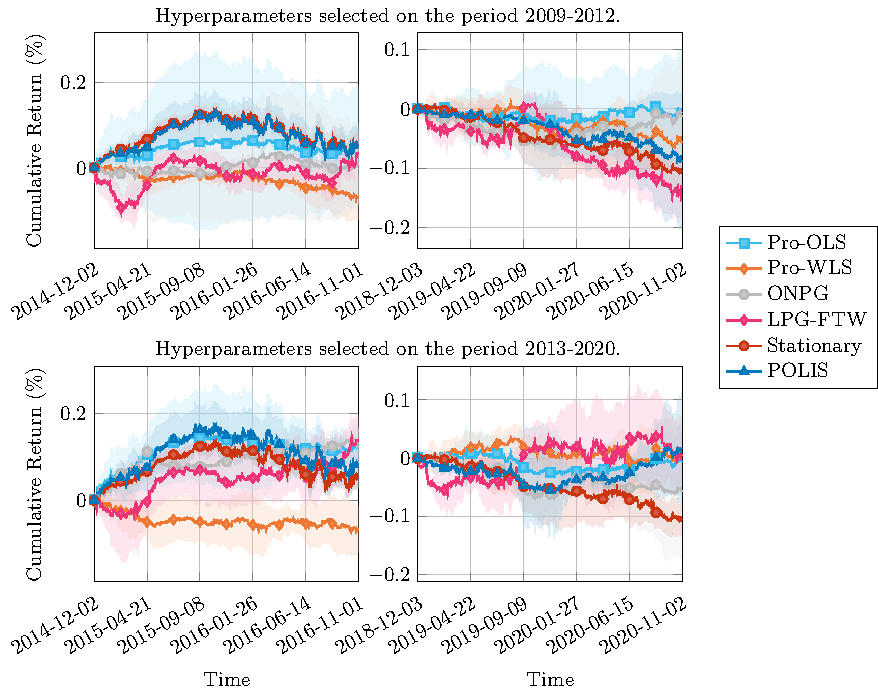
\includegraphics[labellifelongtradingtwo=polistradingeurusd]{img/thesis_plots_chapter_lifelong_trading_2.pdf}
    \caption{两个测试数据集 2013-2016（左）和 2017-2020（右）上 EUR-USD 货币对终身交易的累积回报百分比。注意每个数据集仅显示目标阶段。
    超参数在 2009-2012 期间（上）或 2013-2020 期间（下）选择。
    均值和一倍标准差阴影区域基于 3 个随机种子计算。
    标记对应重新训练步骤的时间。}
    \label{fig:trading_eurusd}
\end{figure}

\noindent\textbf{无延迟 Vasicek 交易.}\indent 在此任务上，我们测试了为 EUR-USD 交易选择的一组超参数。
Vasicek 交易问题的累积回报在 \Cref{fig:trading_vasicek} 中报告。
POLIS 似乎比基线方法更有效地利用了合成资产提供的更清晰信号。它实现了比基线方法更高的最终回报和更小的方差。
特别是，它明显优于平稳策略，后者由于费用而获得了负回报。

作为此环境中的额外实验，我们研究了 POLIS 超参数 $\lambda$（用于方差惩罚的替代正则化项）和 $\beta$（优化中考虑的前视步数）的效果。
我们考虑 $\lambda\in[\![1, 100]\!]$ 和 $\beta\in[\![2, 100]\!]$\footnote{对于 $\beta=1$，\Cref{lem:variance_bound} 中 \Renyi 散度内的左侧项不再涉及分布的混合，可以按照 \cite{papini2019optimistic} 的方式处理。}。
我们感兴趣的是研究 $\lambda$ 和 $\beta$ 如何在回报和奖励标准差之间进行权衡。
结果报告在 \Cref{fig:heatmap_vasicek} 中，表明较小的 $\beta$ 通常产生更高的回报，但代价是
更高的标准差。
$\lambda$ 对此权衡的影响不太明显。
然而，按照设计，该参数允许控制奖励的标准差。

\begin{figure}[t]
    \centering
    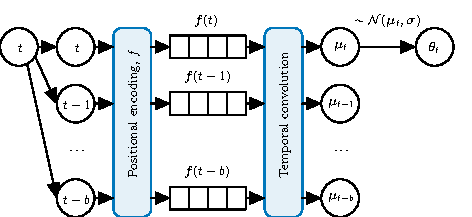
\includegraphics[labellifelongtrading=polisvasicektrading]{img/thesis_plots_chapter_lifelong_trading.pdf}
    \caption{Vasicek 过程上终身交易的累积回报百分比。
    均值和一倍标准差阴影区域基于 10 个随机种子计算。
    标记对应重新训练步骤的时间。}
    \label{fig:trading_vasicek}
\end{figure}

\begin{figure*}[t]
\centering
\begin{subfigure}{.45\textwidth}
  \centering
  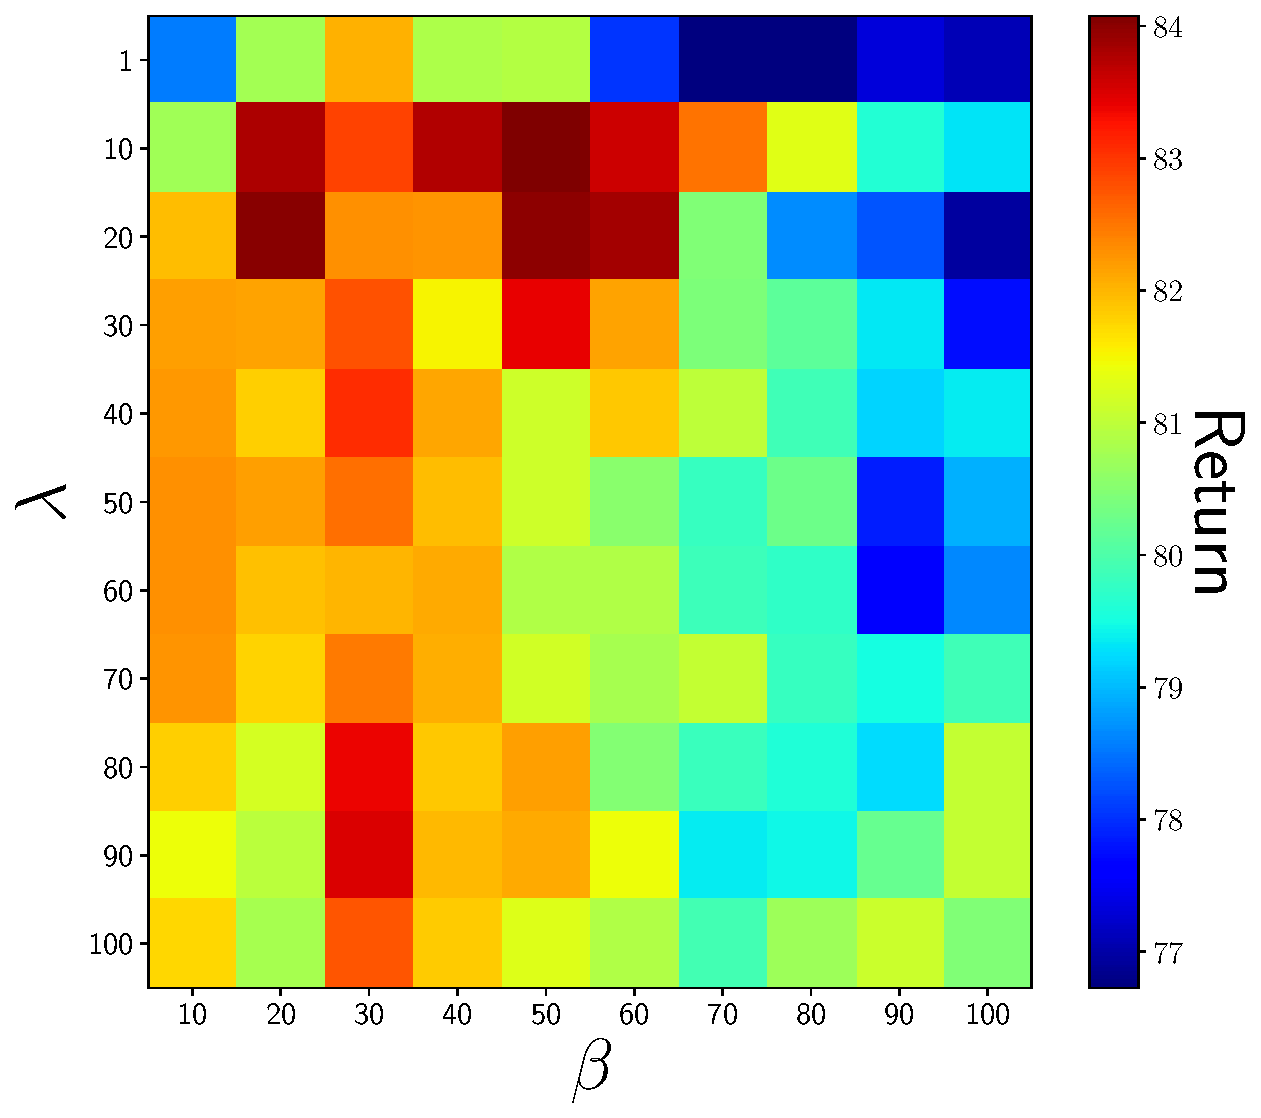
\includegraphics[width=\linewidth]{img/lifelong/vasicek_heatmap_return.pdf}
\end{subfigure}%
\hfill
\begin{subfigure}{.45\textwidth}
  \centering
  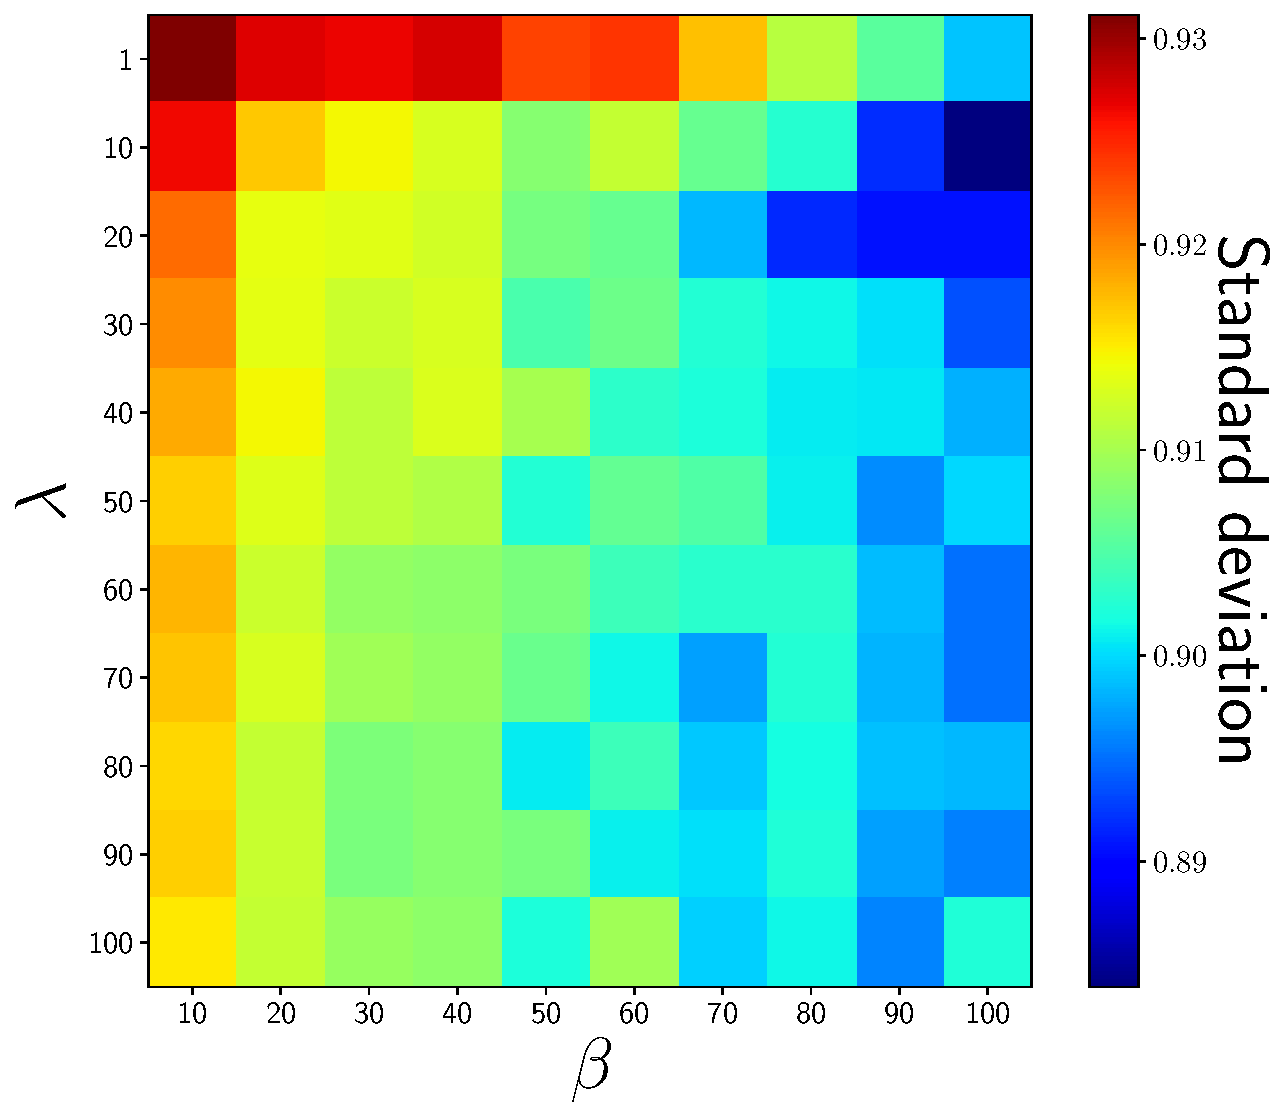
\includegraphics[width=\linewidth]{img/lifelong/vasicek_heatmap_standard_deviation.pdf}
\end{subfigure}%
\hfill
\captionof{figure}{POLIS 在 Vasicek 过程中的回报（左）和奖励标准差（右）随 $\lambda$
和 $\beta$ 的变化。}\label{fig:heatmap_vasicek}
\end{figure*}

\noindent\textbf{无延迟水坝.}\indent 我们在 \Cref{tab:exp_dam} 中报告了实验结果。
令人惊讶的是，在所有基线方法中，平稳超策略在 3 种入流情况下获得了最佳性能。
除平稳策略外，其他基线方法具有较低的回报，并表现出更高标准差的趋势。
POLIS 取得了比这些基线方法好得多的回报，包括方差方面，并与平稳策略持平。
这表明我们的方法能够在不需要额外非平稳性的任务中避免引入多余的非平稳性。

\begin{table}[t]
    \centering
    \begin{tabular}{l|lll}
          & \multicolumn{1}{c}{入流 1}       & \multicolumn{1}{c}{入流 2}        & \multicolumn{1}{c}{入流 3}
        \\ \hline\hline
        Pro-OLS&$-2.6 \pm 0.4$&$-5.2 \pm 5.1$&$-3.8 \pm 0.7$\\
        Pro-WLS&$-5.5 \pm 4.3$&$-8.5 \pm 9.7$&$-8.4 \pm 4.2$\\
        ONPG&$-5.1 \pm 3.2$&$-1.4 \pm 0.2$&$-4.1 \pm 0.5$\\
        LPG-FTW&$-2.3 \pm 0.3$&$-11.9 \pm 8.6$&$-4.7 \pm 1.9$\\
        Stationary&$-2.2 \pm 0.1$&$-1.5 \pm 0.0$&$-3.2 \pm 0.2$\\
        POLIS&$-2.2 \pm 0.2$&$-1.5 \pm 0.0$&$-3.2 \pm 0.2$\\
    \end{tabular}
    \caption{3 种入流情况下水坝环境中的终身学习。目标阶段的平均回报和基于 3 个随机种子的标准差。为美观起见，报告的结果除以 $1e3$ 量级。}\label{tab:exp_dam}
\end{table}


%\begin{table}[t]
%    \centering
%    \begin{tabular}{l|lll}
%          & \multicolumn{1}{c}{Inflow 1}       & \multicolumn{1}{c}{Inflow 2}        %& \multicolumn{1}{c}{Inflow 3}
%        \\ \hline\hline
%        POLIS&$-1.3 \pm 1.0$&$-0.9 \pm 1.2$&$-4.0 \pm 3.2$\\
%        Stationary&$0.0 \pm 0.0$&$-5.3 \pm 0.4$&$-16.7 \pm 0.9$\\
%    \end{tabular}
%    \caption{Lifelong learning on the Dam environment for each of 3 inflow profile %with a longer number of steps between retrains.
%    Mean return on the target period and standard deviation over 3 seeds. Reported %results are divided by an order of $1e3$ for aesthetic.}\label{tab:exp_dam_longer}
%\end{table}





\noindent\textbf{延迟 Vasicek 交易.}\indent 结果在 \Cref{fig:delay_vasicek_trading} 中给出。
正如预期，随着延迟增长，POLIS 的性能下降。
然而，POLIS 对延迟相当鲁棒，即使对于 10 步的较大延迟，也获得了与 \Cref{fig:trading_vasicek} 中最佳无延迟基线方法相似的性能。

\begin{figure}[t]
    \centering
    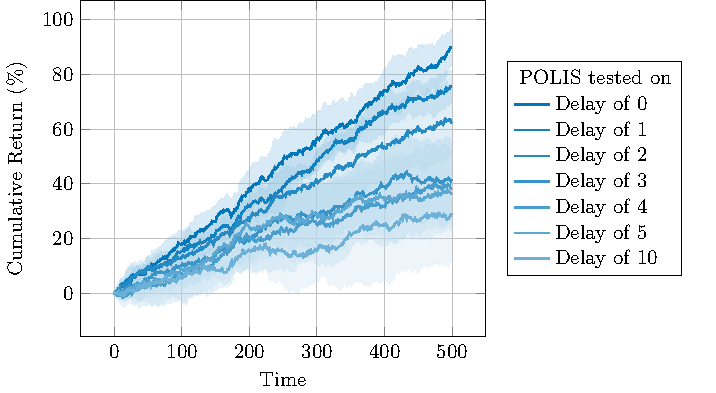
\includegraphics[labellifelongvasicek=polisdelayvasicek]{img/thesis_plots_chapter_lifelong_vasicek.pdf}
    \caption{在 Vasicek 交易环境中以递增延迟运行 POLIS 获得的回报。}
    \label{fig:delay_vasicek_trading}
\end{figure}




\noindent\textbf{延迟水坝.}\indent 水坝延迟测试的结果在 \Cref{tab:exp_dam_delay} 中报告。
延迟对性能有明确的负面影响。
令人惊讶的是，从延迟 1 步到延迟 10 步，性能似乎没有进一步下降。
我们还注意到，延迟对方差似乎没有太大影响，除了第二个入流情况。
POLIS 的性能，即使对于较大的延迟，也与无延迟专家方法的性能相当。

\begin{table}[t]
    \centering
    \begin{tabular}{l|llll}
          POLIS & \multicolumn{1}{c}{无延迟} &
          \multicolumn{1}{c}{延迟 1 步}       & \multicolumn{1}{c}{延迟 5 步}        & \multicolumn{1}{c}{延迟 10 步}
        \\ \hline\hline
        入流 1&$-2.2 \pm 0.2$&$-3.1 \pm 0.3$&$-3.2 \pm 0.2$&$-3.2 \pm 0.2$\\
        入流 2&$-1.5 \pm 0.0$&$-1.4 \pm 0.2$&$-1.5 \pm 0.2$&$-1.5 \pm 0.3$\\
        入流 3&$-3.2 \pm 0.2$&$-4.1 \pm 0.3$&$-4.1 \pm 0.2$&$-4.1 \pm 0.2$\\
    \end{tabular}
    \caption{POLIS 在延迟水坝环境上获得的回报。
    目标阶段的平均回报和基于 3 个随机种子的标准差。
    为美观起见，报告的结果除以 $1e3$ 量级。}\label{tab:exp_dam_delay}
\end{table}
